% Imported from algorithms/diffusion-transformers/README.md
\chapter{时空 DiT 与多模态注意力}\label{seedance-m03}
\moduleinfo{M03}{基础方法与机制解释}{\hyperref[src-seedance-1.0]{\texttt{seedance-1.0}}、\hyperref[src-dit]{\texttt{dit}}、\hyperref[src-video-dit-scaling-laws]{\texttt{video-dit-scaling-laws}}、\hyperref[src-wan-2.1]{\texttt{wan-2.1}}、\hyperref[src-wan21-code]{\texttt{wan21-code}}、\hyperref[src-vincie-code]{\texttt{vincie-code}}}

位置有了定义，再看主干内部的时空注意力怎样组织序列与文本交互。

速度回归的目标已经确定，接下来才是用什么网络表示它。主干读入 VAE 的带噪潜变量，一方面要让画面符合文本，另一方面要让同一物体沿时间连续运动。若把所有时空位置一次全部相连，成本很高；空间与时间解耦的 DiT 就把这两种交互拆到交替执行的注意力层中。

\section{潜变量怎样进入 Transformer}\label{seedance-m03-ux6f5cux53d8ux91cfux600eux6837ux8fdbux5165-transformer}

设视觉潜变量形状为 \codepath{B×C×T×H×W}。将每个网格位置投影到隐藏维度 \(d\)，得到 \codepath{B×T×H×W×d}，再按注意力层需要组织成序列。文本经过编码器后也投影到可交互的特征空间。

这里先分清 token 和通道。有的模型把多个潜位置拼成 patch，有的直接把一个位置当一个 token；后者仍要做输入投影。VAE 给出每个位置存什么，投影决定主干用多宽的特征计算，不能直接把潜通道数当成所有注意力头的维度。

\begin{figure}
\centering
\pandocbounded{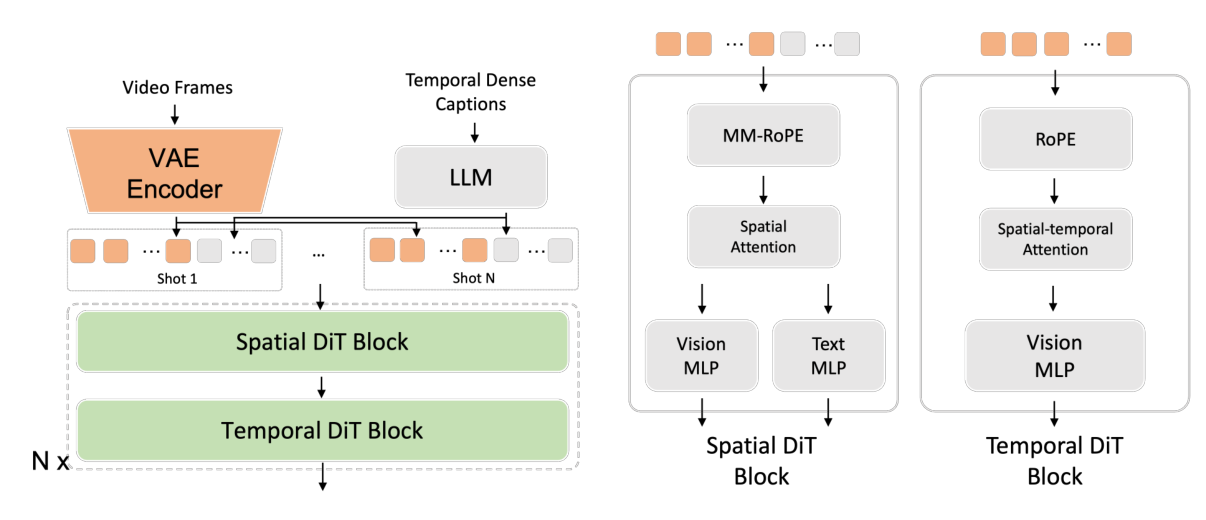
\includegraphics[keepaspectratio,alt={空间层与时间层交替组成的视频生成主干 （论文示意，来源：seedance-1.0）}]{assets/seedance/figures/spatial-temporal-dit.png}}
\caption{空间层与时间层交替组成的视频生成主干 （论文示意，来源：seedance-1.0）}
\end{figure}

按图中的顺序，空间块先让视觉与文本发生交互，时间块再沿视觉序列传播信息。于是文本的语义约束可以先进入画面，随后通过交替的时空计算影响运动。这里的分工来自具体计算图，不能只从“DiT”这个名称判断。

\section{空间层怎样融合文字与画面}\label{seedance-m03-ux7a7aux95f4ux5c42ux600eux6837ux878dux5408ux6587ux5b57ux4e0eux753bux9762}

MMDiT 再把文本也看成可更新的流。视觉与文本各自先经过归一化、QKV 投影和前馈网络，随后沿 token 维拼接，得到：

\[
Q=[Q_v;Q_c],\qquad K=[K_v;K_c],\qquad V=[V_v;V_c].
\]

拼接后，两种模态的 query 都能读取联合的 key/value，因此一次自注意力写为：

\[
Y=\operatorname{softmax}\left(\frac{QK^\top}{\sqrt{d_h}}+A\right)V.
\]

从这个式子还可以按行拆回视觉与文本输出。两种模态都给 query，就都取得更新；它们的参数仍可各自独立。因此“特征先分路、注意力时拼接”和“所有层都共享参数”不是同一个意思。

\(d_h\) 是单头维度，\(A\) 是可见性掩码。视觉 query 可以读取文本 key/value，文本 query 也能读取视觉 key/value；输出再拆回两种模态，各自经过投影、残差和前馈网络。

从输出的 query 行就能看出区别。单向文本 cross-attention 通常由视觉给 query，文本只给 key/value，因此只返回视觉序列；联合自注意力则也返回文本对应的更新。说“文本作为条件”还不够，必须继续说明文本在这次计算中究竟是哪一种角色。

反向传播也沿这整张计算图进行，不存在先看 Q、再看 K、最后看 V 的重要性排序。哪些参数更新，要看梯度路径和冻结设置。Q/K normalization 另用于控制注意力的数值尺度，与文本是否产生 query 是两个问题。

\section{时间层存在两种不同的组织方式}\label{seedance-m03-ux65f6ux95f4ux5c42ux5b58ux5728ux4e24ux79cdux4e0dux540cux7684ux7ec4ux7ec7ux65b9ux5f0f}

设每帧有 \(P=HW\) 个空间位置。最便宜的时间注意力，把同一位置在所有帧上的 token 串起来，序列形状为 \codepath{B×P} 组长度为 \(T\) 的序列。它能直接关联某个位置的时间变化，但一个物体移动到邻近位置后，需要其它空间层帮助传递信息。

另一种做法是在每帧划分空间窗口，窗口含 \(m\) 个位置，把同一窗口跨所有帧的 token 合并，形成 \(P/m\) 组长度为 \(Tm\) 的序列。这样一次注意力可以同时看到时间变化和窗口内位移。

{\def\LTcaptype{table} % do not increment counter
\small\setlength{\tabcolsep}{3pt}\renewcommand{\arraystretch}{1.18}
\begin{longtable}[]{@{}
  >{\raggedright\arraybackslash}p{(\linewidth - 4\tabcolsep) * \real{0.1900}}
  >{\raggedright\arraybackslash}p{(\linewidth - 4\tabcolsep) * \real{0.3900}}
  >{\raggedright\arraybackslash}p{(\linewidth - 4\tabcolsep) * \real{0.4200}}@{}}
\toprule\noalign{}
\begin{minipage}[b]{\linewidth}\raggedright
组织方式
\end{minipage} & \begin{minipage}[b]{\linewidth}\raggedright
注意力输入形状
\end{minipage} & \begin{minipage}[b]{\linewidth}\raggedright
可直接交互的范围
\end{minipage} \\
\midrule\noalign{}
\endhead
\bottomrule\noalign{}
\endlastfoot
逐位置时间注意力 & \codepath{B×P, T, d} & 一个空间位置上的所有帧 \\
窗口时空注意力 & \codepath{B×(P/m), Tm, d} & 一个空间窗口内的所有帧与位置 \\
\end{longtable}
}

从 \codepath{B,T,nwin,m,d} 出发，窗口时空形式先重排成 \codepath{B,nwin,T,m,d}，再合并 \(T\) 和 \(m\)。如果把 \(m\) 合进 batch，得到的依然是逐位置时间注意力，并没有窗口内空间交互。

\section{复杂度为什么要乘回帧数和位置数}\label{seedance-m03-ux590dux6742ux5ea6ux4e3aux4ec0ux4e48ux8981ux4e58ux56deux5e27ux6570ux548cux4f4dux7f6eux6570}

下面暂时不计投影和前馈，只数一个注意力头中的 token 连接。把每种序列有多长、重复几组写出来，成本就比较清楚了：

\[
\begin{aligned}
C_{\mathrm{full}}&=(TP)^2,\\
C_{\mathrm{spatial}}&=TP^2,\\
C_{\mathrm{temporal}}&=PT^2,\\
C_{\mathrm{window}}&=\frac{P}{m}(Tm)^2=PT^2m.
\end{aligned}
\]

空间加逐位置时间注意力的总成本是 \(TP^2+PT^2\)。帧内空间注意力要做 \(T\) 次，逐位置时间注意力要做 \(P\) 次，这两个重复次数不能省略。若使用窗口时空形式，时间项还要乘窗口面积 \(m\)。

取 \(T=16\)、\(H=W=32\)、\(P=1024\)、\(m=4\)，全时空有约 2.68 亿个连接，空间项约 1678 万，逐位置时间项约 26 万，窗口时空项约 105 万。连接数的大幅下降解释了结构化注意力的价值，但真实速度还受投影、前馈网络、kernel 和显存访问影响。

在乘加计为两次操作的约定下，标准 MHA 子层的粗略 FLOPs 为：

\[
8Nd^2+4N^2d.
\]

前一项来自 QKV 和输出投影，后一项来自 QK 与 AV；扩展比例为 \(r\) 的普通两层 FFN 另需约 \(4rNd^2\)。GQA 减少 K/V 头数，能降低投影和缓存开销，但每个 query 头仍然计算自己的注意力，二次交互项不会自动消失。

\section{输入变大，为什么权重可以不变}\label{seedance-m03-ux8f93ux5165ux53d8ux5927ux4e3aux4ec0ux4e48ux6743ux91cdux53efux4ee5ux4e0dux53d8}

线性层作用于最后的特征维度 \(d\)，权重不含 token 数 \(N\)。增加分辨率主要增加 token 行数，因此参数形状可以保持不变；LayerNorm 的参数同样沿特征维度定义。

不过，参数形状能复用，只回答了网络能否计算。位置范围变大、宽高比改变、物体跨窗口移动，以及长序列训练分布不同，都还会影响生成。因而分辨率适配要接着看算力与结果质量，前向不报错只是其中一步。

\section{从极简代码到真实实现}\label{seedance-m03-ux4eceux6781ux7b80ux4ee3ux7801ux5230ux771fux5b9eux5b9eux73b0}

注意力的区别首先体现在谁成为序列维。输入为 \codepath{B,T,H,W,d} 时，逐位置时间形式可以写成：

\begin{verbatim}
b, t, h, w, d = x.shape
seq = x.permute(0, 2, 3, 1, 4).reshape(b*h*w, t, d)
y = attention(seq)  # 每组只读同一位置的 T 个时间点。
\end{verbatim}

窗口时空形式则把一个窗口的时间与空间位置一起合并为长度 \(Tm\)。两种 reshape、逆变换和多模态拼接见 \hyperref[code-attention-layout]{attention\_layout.py}。真实投影与 block 可读 \href{https://github.com/Wan-Video/Wan2.1/blob/9737cba9c1c3c4d04b33fcad41c111989865d315/wan/modules/model.py}{Wan 模型}，多模态窗口实现可读 \href{https://github.com/ByteDance-Seed/VINCIE/blob/97cd2c5701e694dabcfea320c0cf59893d427fab/models/dit/blocks/attention/mmattn.py}{VINCIE attention}；它们是不同基座的结构，不能混用 checkpoint。
